\begin{itemize}
	\item ограничить сечение рассеяния можно зная: конечное распределение ($aT_{\odot}^2$), ограничение на темп аннигиляции  $A$ из нейтриного сигнала. 
\end{itemize}
\begin{figure}[!h]
	\centering
	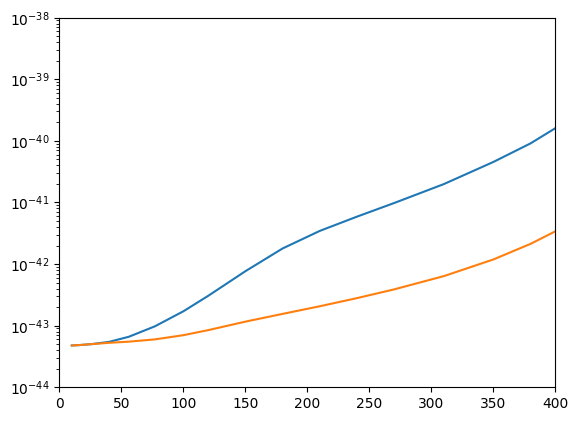
\includegraphics[width=0.65\textwidth]{images/Constrains.png}
	\caption{Пример ограничений из данных IceCube в канале $\chi+\chi \to W^{+} + W^{-}$}
\end{figure}